\documentclass[12pt,a4paper]{article}

\usepackage[T1]{fontenc}
\usepackage[utf8]{inputenc}
\usepackage{geometry}
\usepackage{amsmath}
\usepackage{booktabs}
\usepackage{hyperref}
\usepackage{parskip}
\usepackage{microtype}
\usepackage{caption}
\usepackage{float}
\usepackage{tikz}
\usepackage{enumitem}
\usetikzlibrary{shapes.geometric, arrows.meta, positioning, backgrounds}

\geometry{margin=1.2in}

% ── TikZ flowchart styles ────────────────────────────────────────────────────
\tikzset{
  block/.style    = {rectangle, rounded corners, draw=black, fill=blue!8,
                     text width=7.5cm, minimum height=1cm, align=center,
                     font=\small},
  decision/.style = {diamond, draw=black, fill=orange!15,
                     text width=3.0cm, align=center, font=\small,
                     inner sep=1pt},
  startend/.style = {rectangle, rounded corners=8pt, draw=black, fill=gray!20,
                     text width=4.5cm, minimum height=1cm, align=center,
                     font=\small\bfseries},
  arrow/.style    = {-{Stealth[length=2mm]}, thick},
  notelabel/.style= {font=\footnotesize},
}

% ── Document metadata ────────────────────────────────────────────────────────
\title{%
  \textbf{CAN Bus Motor Control}\\[0.5em]
  \large Communication Architecture for the AK60-6 Motor\\
  \normalsize Lower Exosuit --- Motor Module
}
\author{Exosuit Team}
\date{February 2026}

\begin{document}

\maketitle
\tableofcontents
\newpage

% ═══════════════════════════════════════════════════════════════════════════
\section{Introduction}

This chapter describes how the exosuit communicates with the AK60-6 motor
manufactured by CubeMars. The focus is on the communication interface
chosen, the reasoning behind that choice, and the mechanisms developed
to make the motor respond reliably to movement commands.

The explanation is written to be accessible to a reader who is not familiar
with low-level hardware communication. Technical terms are introduced and
explained when they first appear.

% ═══════════════════════════════════════════════════════════════════════════
\section{Choosing the Right Communication Interface}
\label{sec:motivation}

The AK60-6 motor supports two ways of receiving commands from a computer.
The first is called UART (Universal Asynchronous Receiver--Transmitter),
a simple point-to-point serial link. The concept is similar to plugging
a keyboard directly into a computer: one cable connects one motor to the
computer, and commands are exchanged over that single dedicated link.

The second option is CAN Bus (Controller Area Network). Originally developed
for the automotive industry, CAN is a robust two-wire network that allows
many devices to share the same pair of wires simultaneously. Each device on
the network is identified by a unique address, and a message is only acted
upon by the device whose address matches the one in the message.

The project began with UART because it is straightforward to set up.
As development progressed, several reasons made CAN the clearly superior
choice for this application.

\subsection{Physical Incompatibility Discovered During Development}

The most important finding during development was that the UART cable and
the CAN bus \emph{cannot be connected to the motor at the same time}. When
the UART cable was plugged in alongside CAN, the motor's status broadcasts
over the CAN network stopped completely and silently. The moment the UART
cable was physically removed, the broadcasts resumed immediately.

This is a hardware-level conflict inside the motor: the electronics for UART
communication interferes with the CAN receiver when both are powered
simultaneously. The practical consequence is that a single interface must
be chosen --- the two cannot coexist on this motor.

\subsection{Wiring Scalability}

UART requires a dedicated pair of wires between the computer and each
individual motor. Since the exosuit has multiple motors per limb, a
UART-based design would require a large number of separate cables, adding
weight, bulk, and mechanical complexity to a device that must be worn
comfortably.

CAN requires only one shared pair of wires --- the CAN bus --- that all
motors connect to in parallel. The computer places a message on this shared
wire, and only the motor whose address matches the message will act on it.
This is analogous to a public address system where each seat in an
auditorium has a number: only the person in the called seat stands up,
while everyone else ignores the announcement.

\subsection{Resistance to Electrical Noise}

The CAN standard uses a technique called \emph{differential signalling}.
Rather than sending a signal on one wire relative to a shared ground, CAN
transmits the same signal simultaneously on two wires but with opposite
polarities. The receiving device looks only at the \emph{difference} in
voltage between the two wires.

Any electrical noise that is picked up along the cable affects both wires
equally and therefore cancels out in the difference. In an exosuit, motors,
power electronics, and signal cables are in very close physical proximity.
Rapidly switching motor currents generate electromagnetic interference that
can corrupt nearby signals. Differential signalling makes CAN inherently
immune to this type of noise, whereas UART, which uses a single signal wire
relative to ground, is susceptible to it.

\subsection{Message Prioritisation}

On a CAN network, every message carries a priority level encoded in its
address. If two devices attempt to send a message at the same moment, the
network hardware automatically resolves the conflict and allows the
higher-priority message through first, without either message being lost
or corrupted.

This property guarantees that a high-priority command such as an emergency
stop will always reach all motors promptly, regardless of what other
messages are in transit at the time. UART provides no equivalent
mechanism.

% ═══════════════════════════════════════════════════════════════════════════
\section{Hardware Setup}
\label{sec:hardware}

The on-board computer used in this system is the NVIDIA Jetson Orin AGX.
It contains a built-in CAN controller, but requires a small external chip
called a CAN transceiver to convert the controller's internal logic signals
into the differential voltage levels used on the physical bus.

\subsection{Electrical Termination}

For CAN to operate reliably at high speed, the bus wires must be terminated
at both physical ends of the cable with a $120\,\Omega$ resistor. This
resistor absorbs electrical reflections that would otherwise travel back
along the wire and corrupt data. The AK60-6 motor has a built-in
terminator. The Jetson CAN transceiver board must also have its own
terminator enabled via a jumper or solder bridge. If either terminator
is missing, communication will be unreliable at the 1\,Mbit/s speed
required by the motor.

\subsection{Interface Configuration Parameters}

Before the Jetson can send any messages, its operating system must be
instructed to activate the CAN interface with the correct settings.
Three parameters are configured at system startup:

\begin{description}[leftmargin=3.5cm, style=nextline]
  \item[Bus speed] The network must operate at exactly 1\,Mbit/s (one
    million bits per second). All devices on the bus must use the same
    speed. A mismatch means no device will receive any messages. This
    speed is fixed by the motor manufacturer's specification.

  \item[Error reporting] The interface is configured so that hardware
    faults --- such as a broken wire or corrupted message --- are made
    visible to the software layer. Without this setting, a physical
    wiring problem would produce no observable error and would be
    extremely difficult to diagnose.

  \item[Automatic recovery] The CAN standard requires a device that
    encounters too many consecutive errors to enter a protective state
    called \emph{bus-off}, where it stops transmitting entirely.
    A recovery timer is configured so that the interface automatically
    exits this state every 100\,milliseconds. This makes the system
    self-healing after a transient electrical fault, without requiring
    manual intervention.
\end{description}

% ═══════════════════════════════════════════════════════════════════════════
\section{How Commands Are Sent to the Motor}
\label{sec:protocol}

\subsection{The Structure of a CAN Message}

Every message on a CAN network consists of two parts: an \emph{address}
(also called the arbitration ID) and a \emph{payload}. The address tells
every device on the shared bus who the message is for and what kind of
instruction it contains, without the devices needing to read the payload.
The payload carries the numerical value associated with the instruction.

\subsection{Encoding the Instruction Type into the Address}

CubeMars uses an extended address format that packs two independent pieces
of information into a single address number:

\begin{itemize}
  \item The \textbf{upper portion} of the address encodes the
        \emph{type of instruction} --- for example, ``set velocity'',
        ``set position'', or ``set current''.
  \item The \textbf{lower portion} of the address encodes the
        \emph{motor's unique identification number}.
\end{itemize}

The two values are combined using a standard binary packing operation.
For a motor with identification number~3 receiving a velocity command
(instruction type~3), the resulting address is:

\begin{equation}
  \text{Address} = (\text{instruction type} \times 256) + \text{motor ID}
  = (3 \times 256) + 3 = 771
\end{equation}

Every device on the shared bus sees this address, but only the motor with
identification number~3 recognises it as relevant and processes the payload.
All other devices ignore it.

\subsection{Available Instruction Types}

Table~\ref{tab:modes} lists the instruction types that the motor supports.
Each type accepts a numerical setpoint in the payload, which must be
converted into an integer representation using a defined scale factor
before transmission.

\begin{table}[H]
  \centering
  \caption{Supported motor control instruction types}
  \label{tab:modes}
  \begin{tabular}{p{3.8cm} p{5.0cm} p{4.0cm}}
    \toprule
    Instruction Type & What it controls & How the value is encoded \\
    \midrule
    Duty Cycle
      & The fraction of supply voltage applied to the motor windings,
        similar to a throttle percentage between $-1$ (full
        reverse) and $+1$ (full forward).
      & Desired fraction multiplied by 100\,000;
        stored as a 32-bit integer. \\[6pt]
    Current Control
      & The electrical current flowing through the windings, which
        is directly proportional to the torque the motor produces.
      & Desired current in Amperes multiplied by 1\,000;
        stored as a 32-bit integer. \\[6pt]
    Velocity Control
      & The rotational speed of the motor shaft, expressed in
        electrical RPM.
      & Desired electrical RPM sent directly as a 32-bit integer,
        with no additional scaling. \\[6pt]
    Position Control
      & The absolute angular position of the motor shaft in degrees.
      & Desired angle in degrees multiplied by 10\,000;
        stored as a 32-bit integer. \\[6pt]
    Position with Speed Limit
      & A target position with an upper limit on how fast the motor
        may travel to reach it, and how quickly it may accelerate.
      & Target position as above. Speed and acceleration limits are
        each divided by 10 before being stored as 16-bit integers. \\
    \bottomrule
  \end{tabular}
\end{table}

All payloads are padded with zeros to a total length of exactly 8 bytes,
as required by the protocol. All integer values are stored in big-endian
byte order (most significant byte first), which is the network standard.

\subsection{Enabling and Disabling the Motor}

Before the motor will respond to any movement command, it must be
explicitly enabled via a dedicated activation message. This is a
deliberate safety feature: the motor will not move on power-up until the
computer intentionally sends the enable command. A corresponding
deactivation message returns the motor to a free-spinning, unpowered state.
These two messages use unique data patterns that cannot be confused with
any normal control command.

\subsection{A Scaling Error Discovered and Corrected}

During testing of the Position with Speed Limit mode, a discrepancy between
the commanded speed and the actual motor behaviour was observed. On
investigation, the protocol specification states that the speed and
acceleration limits in this mode must be divided by ten before being placed
in the message. The initial software implementation had omitted this
division step, meaning that a requested speed limit of 10\,000 electrical
RPM was actually commanding 100\,000 electrical RPM --- ten times the
intended value. The correction was straightforward: apply the division by
ten before constructing the message.

% ═══════════════════════════════════════════════════════════════════════════
\section{How the Motor Reports Its State}
\label{sec:feedback}

\subsection{Automatic Status Broadcasts}

While the motor is active, it continuously broadcasts a status message onto
the CAN bus at a rate of 50 messages per second (one every 20
milliseconds). The computer receives these messages passively and uses them
to maintain an up-to-date picture of the motor's condition without needing
to request information explicitly.

Each status message carries the five fields listed in
Table~\ref{tab:feedback}.

\begin{table}[H]
  \centering
  \caption{Information contained in each motor status broadcast}
  \label{tab:feedback}
  \begin{tabular}{p{3.0cm} p{5.5cm} p{4.2cm}}
    \toprule
    Field & Meaning & Conversion to real units \\
    \midrule
    Position
      & Current angular position of the shaft, relative to the
        origin set at startup.
      & Received integer value multiplied by $0.1$ gives degrees. \\[6pt]
    Speed
      & Current rotational speed of the shaft.
      & Received integer value multiplied by $10$ gives electrical
        RPM. \\[6pt]
    Current
      & Electrical current flowing through the motor windings,
        which reflects the torque being produced.
      & Received integer value multiplied by $0.01$ gives
        Amperes. \\[6pt]
    Temperature
      & Temperature of the motor driver electronics.
      & Integer value read directly in degrees Celsius. \\[6pt]
    Error Code
      & A number indicating any active fault condition detected
        by the motor's own firmware.
      & Zero means no fault. Non-zero values encode specific error
        types as defined in the manufacturer's documentation. \\
    \bottomrule
  \end{tabular}
\end{table}

\subsection{Verifying Communication During Development}

Early in development, before any movement commands were issued, a passive
listening tool was used to display all traffic on the CAN bus in a
human-readable form. The system was considered to be communicating correctly
only when status messages from the motor appeared at a consistent 50\,Hz
rate.

This verification step was what revealed the UART cable hardware conflict
described in Section~\ref{sec:motivation}. The status broadcasts were
completely absent as long as the UART cable was connected. The moment it
was disconnected, the broadcasts appeared immediately and consistently,
resolving what had been an unexplained communication failure.

% ═══════════════════════════════════════════════════════════════════════════
\section{The Motor Watchdog and the Continuous Refresh Mechanism}
\label{sec:watchdog}

\subsection{The Watchdog Timer}

The AK60-6 motor firmware incorporates a safety feature called a
\emph{watchdog timer}. This mechanism monitors how recently the motor
received a command from the computer. If no command arrives within
approximately 100\,milliseconds, the motor automatically cuts power to
its drive output and the shaft coasts to a stop.

The purpose is to protect against a scenario where the control computer
crashes, or the communication cable becomes disconnected, while the motor
is in motion. Without this protection, the motor would continue executing
its last command indefinitely, which could be dangerous in a wearable
device. The watchdog ensures that loss of communication results in the
motor stopping within 100\,milliseconds.

\subsection{The Problem This Created in the Initial Implementation}

In the initial implementation, each time a control instruction was issued
--- such as ``set velocity to 5\,000 RPM'' --- exactly one message was
transmitted over the CAN bus. That single message would satisfy the
watchdog once, causing the motor to activate. However, because no further
messages arrived within the 100\,millisecond window, the watchdog would
then cut the power and the motor would stop. The observable effect was a
brief mechanical twitch lasting roughly 100\,milliseconds, rather than
sustained motion. Issuing another command produced another twitch.

\subsection{The Solution: Continuous Command Repetition}

The solution is to repeat the active command continuously at a rate faster
than the watchdog timeout. The chosen rate is 50 repetitions per second
(one every 20\,milliseconds), providing a safety margin of five times over
the watchdog threshold.

To avoid requiring the programmer to manually manage a timing loop every
time they issue a command, a \emph{background process} was implemented.
This is a separately running task that operates invisibly alongside the
main program. Its sole responsibility is to keep retransmitting the most
recently issued command at the required rate. The programmer does not
interact with it directly.

Figure~\ref{fig:refresh} illustrates how this mechanism works.

\begin{figure}[H]
  \centering
  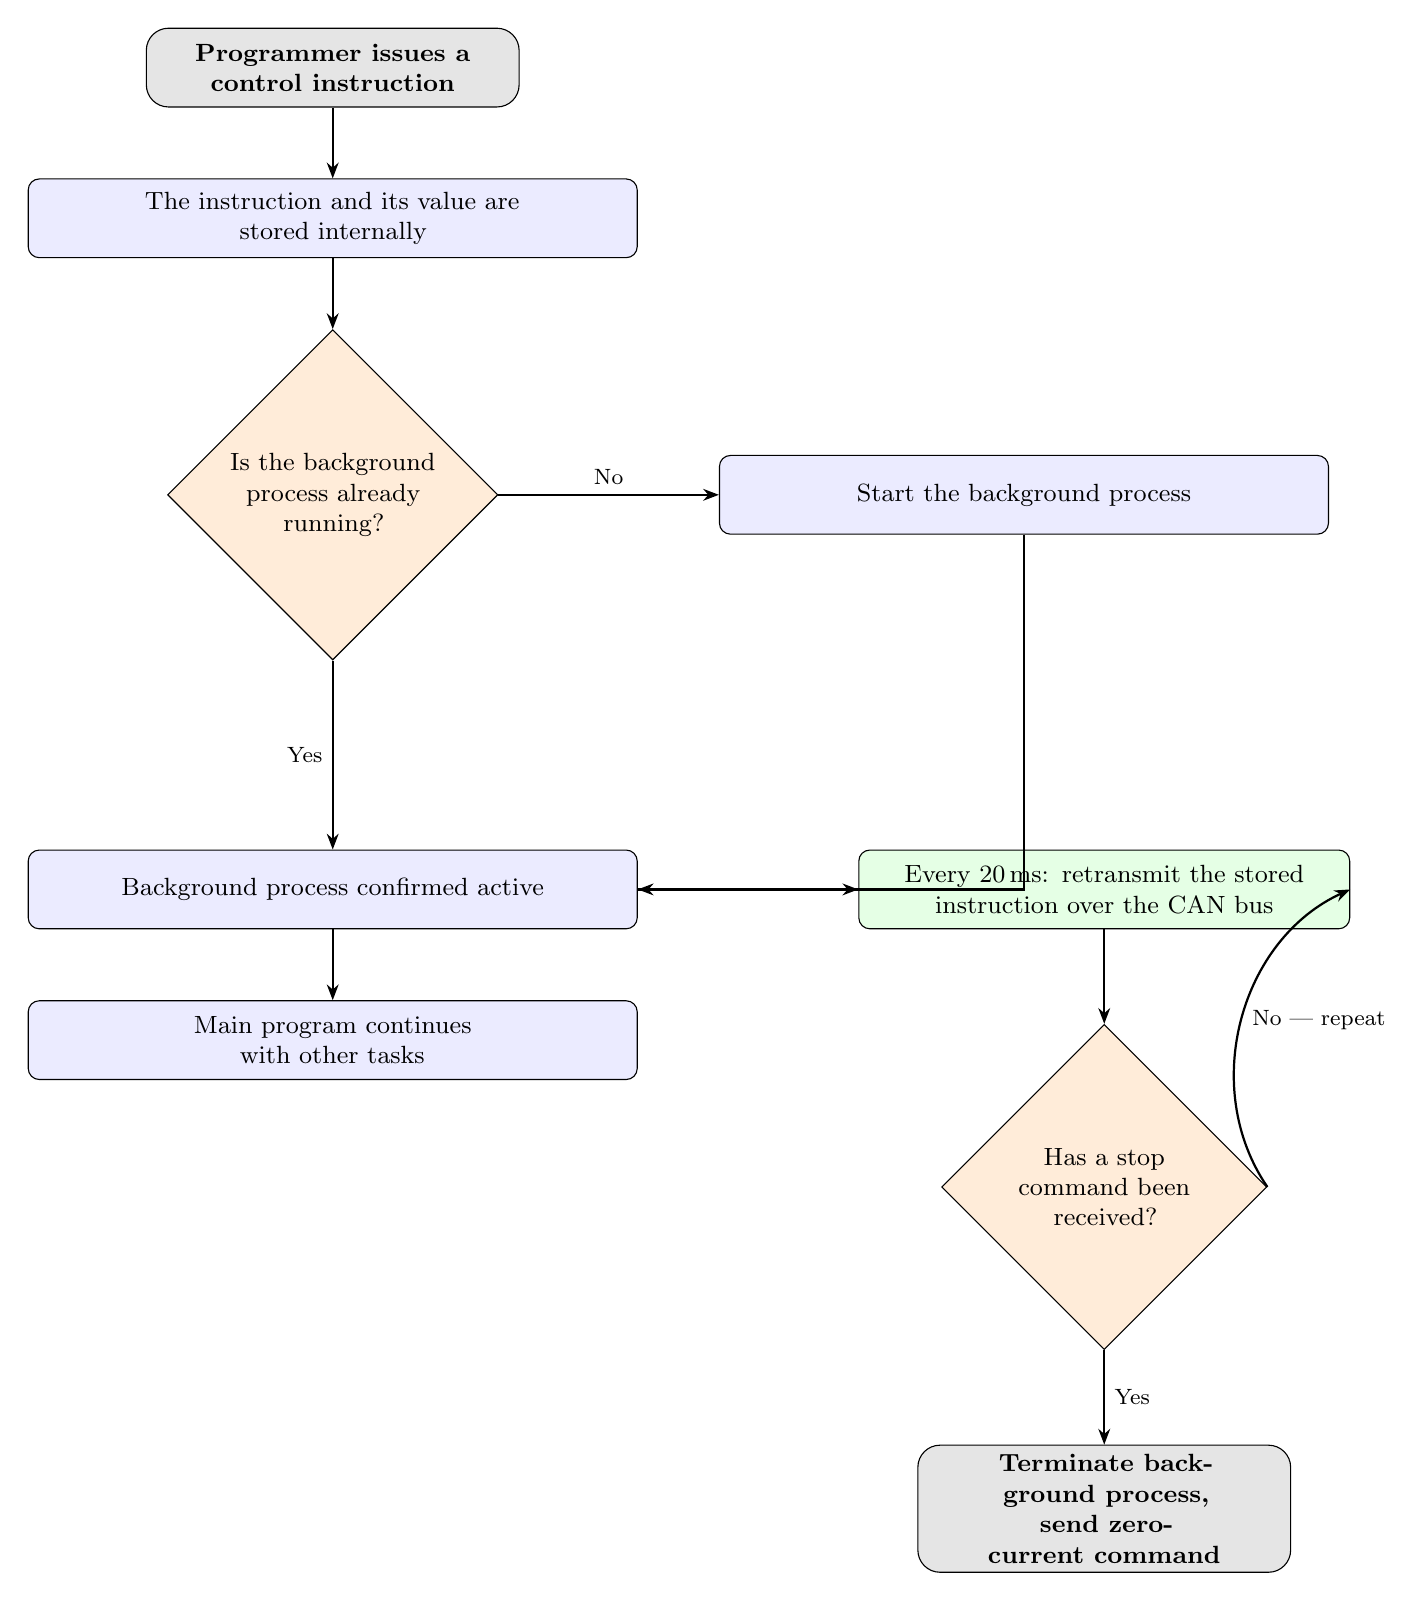
\begin{tikzpicture}[node distance=0.9cm and 2.2cm]

    % ── Left column: main program ─────────────────────────────────
    \node[startend] (start)
      {Programmer issues a\\ control instruction};

    \node[block, below=of start] (store)
      {The instruction and its value are\\ stored internally};

    \node[decision, below=of store] (running)
      {Is the background\\process already\\running?};

    \node[block, right=2.8cm of running] (launch)
      {Start the background process};

    \node[block, below=2.4cm of running] (ready)
      {Background process confirmed active};

    \node[block, below=of ready] (main)
      {Main program continues\\ with other tasks};

    % ── Right column: background loop ─────────────────────────────
    \node[block, right=2.8cm of ready, fill=green!10,
          text width=6cm] (loop)
      {Every 20\,ms: retransmit the stored\\ instruction over the CAN bus};

    \node[decision, below=1.2cm of loop] (stop)
      {Has a stop\\ command been\\ received?};

    \node[startend, below=1.2cm of stop] (end)
      {Terminate background process,\\ send zero-current command};

    % ── Arrows ────────────────────────────────────────────────────
    \draw[arrow] (start)   -- (store);
    \draw[arrow] (store)   -- (running);
    \draw[arrow] (running) -- node[notelabel, above]{No} (launch);
    \draw[arrow] (launch)  |- (ready);
    \draw[arrow] (running) -- node[notelabel, left]{Yes} (ready);
    \draw[arrow] (ready)   -- (main);
    \draw[arrow] (ready.east) -- (loop.west);
    \draw[arrow] (loop)    -- (stop);
    \draw[arrow] (stop.east) to[bend left=50]
                 node[notelabel, right]{No --- repeat} (loop.east);
    \draw[arrow] (stop)    -- node[notelabel, right]{Yes} (end);

  \end{tikzpicture}
  \caption{The continuous command refresh mechanism. When an instruction
           is issued (left column), a background process is started or updated
           (right column) that retransmits the instruction every 20\,ms.
           This keeps the motor's watchdog satisfied indefinitely. When stop
           is commanded, the background process is terminated and a
           zero-current command signals the motor to release.}
  \label{fig:refresh}
\end{figure}

When a new instruction is issued while the background process is already
running --- for example, changing from one speed to another --- the stored
value is simply updated. The background process picks up the new value on
its next 20\,millisecond cycle without needing to be restarted.

When a stop command is received, the background process is terminated
first, and then a zero-current command is sent directly to the motor.
Applying zero current releases the motor windings completely, allowing the
shaft to coast to a mechanical stop. Sending the stop command through the
background process would have been counterproductive, as it would have
started a refresh loop holding zero current rather than cleanly terminating all activity.

\subsection{First Confirmed Motor Movement}

The approach was first validated with a standalone test script before being
integrated into the main control software. A duty cycle value of 20\,\%
(meaning the motor receives one fifth of the full supply voltage) was
issued and retransmitted continuously for two seconds.

During this test, the motor's own status broadcasts reported a steady
rotational speed of approximately 3\,400 electrical RPM throughout the
two-second window. The shaft angular position, as reported in the feedback,
increased from approximately $7.5^\circ$ to $519.6^\circ$ --- just under
one and a half full revolutions. The monotonically increasing position
confirmed that motion was sustained for the full duration and was not a
brief transient.

% ═══════════════════════════════════════════════════════════════════════════
\section{Soft-Start: Managing the Low-Speed Noise Zone}
\label{sec:softstart}

\subsection{Observed Problem at Low Speeds}

During initial testing of the velocity control mode, an unexpected behaviour
was observed when the motor was commanded to accelerate from rest. At low
speeds --- specifically in the range from zero up to approximately 5\,000
electrical RPM --- the motor produced an audible high-pitched noise and the
measured current showed rapid oscillations.

The cause is the velocity controller built into the motor's own firmware.
This controller uses a fixed, aggressive acceleration profile to bring the
motor up to speed. At low speeds, this aggressive acceleration causes the
current to overshoot and undershoot its target value repeatedly, producing
the oscillations. The effect is both acoustically undesirable and
mechanically harmful over repeated cycles, as it introduces vibration into
the drivetrain.

\subsection{The Soft-Start Approach}

To avoid this behaviour, a preparatory step called \emph{soft-start} was
added. Before any velocity command is executed, the control system
temporarily switches the motor into current control mode and applies a
modest, fixed current of 3\,000\,milliamperes.

In current control mode, there is no velocity feedback loop. The motor
simply receives a torque-producing current and accelerates gradually and
smoothly. The noisy low-speed zone is traversed under this gentle torque
without the aggressive velocity controller being active. After
150\,milliseconds --- sufficient time for the motor to build speed past
the problematic zone --- the system switches into velocity control mode.
By this point, the shaft is already moving at a speed above the oscillation
threshold and the velocity controller takes over smoothly.

The soft-start current of 3\,000\,milliamperes was chosen to be large
enough to reliably accelerate the motor within the allotted time, while
remaining well within the motor's continuous current rating to avoid thermal
stress.

Figure~\ref{fig:softstart} shows the sequence of events during a velocity
command with soft-start.

\begin{figure}[H]
  \centering
  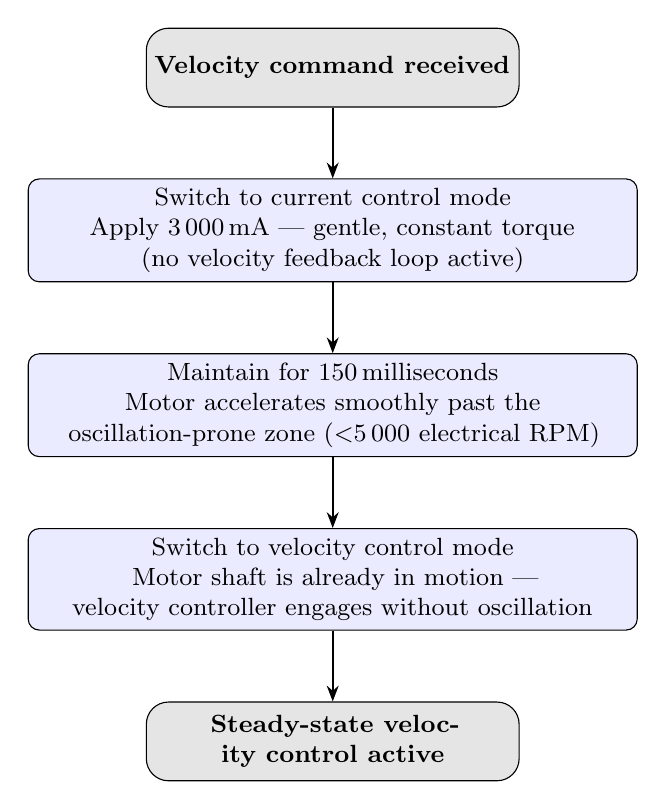
\begin{tikzpicture}[node distance=0.9cm]

    \node[startend] (cmd)
      {Velocity command received};

    \node[block, below=of cmd]
      (current)
      {Switch to current control mode\\
       Apply 3\,000\,mA --- gentle, constant torque\\
       (no velocity feedback loop active)};

    \node[block, below=of current]
      (wait)
      {Maintain for 150\,milliseconds\\
       Motor accelerates smoothly past the\\
       oscillation-prone zone ($<$5\,000 electrical RPM)};

    \node[block, below=of wait]
      (velocity)
      {Switch to velocity control mode\\
       Motor shaft is already in motion ---\\
       velocity controller engages without oscillation};

    \node[startend, below=of velocity]
      (steady)
      {Steady-state velocity control active};

    \draw[arrow] (cmd)     -- (current);
    \draw[arrow] (current) -- (wait);
    \draw[arrow] (wait)    -- (velocity);
    \draw[arrow] (velocity)-- (steady);

  \end{tikzpicture}
  \caption{Soft-start sequence. The first 150\,ms of every velocity command
           uses direct current control (pure torque, no velocity feedback loop)
           to carry the motor shaft past the low-speed oscillation zone before
           the velocity controller is engaged.}
  \label{fig:softstart}
\end{figure}

% ═══════════════════════════════════════════════════════════════════════════
\section{Executing Position Moves}
\label{sec:position}

When the exosuit must move the motor to a specific target angle, a two-phase
strategy is used that combines velocity control with position hold.

\subsection{Phase One: Velocity Travel}

In the first phase, the motor is commanded to run at a specified velocity
in the direction of the target angle. The duration of this phase is
estimated by calculating how long it would take to travel the required
angular distance at the given speed.

The current angular position, obtained from the motor's own 50\,Hz status
broadcasts, is used as the starting point. The conversion from rotational
speed to angular travel rate follows from first principles: one full
revolution per minute corresponds to $360^\circ$ per $60\,\text{s}$, so
the angular speed in degrees per second is:

\begin{equation}
  \omega \,[\text{deg/s}]
  = \frac{\text{Speed [electrical RPM]}}{60} \times 360
\end{equation}

The estimated travel time is then simply the angular distance divided by
the angular speed:

\begin{equation}
  t_{\text{travel}} \,[\text{s}]
  = \frac{\lvert \theta_{\text{target}} - \theta_{\text{current}} \rvert \,[\text{deg}]}
         {\omega \,[\text{deg/s}]}
\end{equation}

This estimate is capped at a maximum permitted movement duration as a
safety measure, preventing the motor from running indefinitely if the
estimate is inaccurate.

\subsection{Phase Two: Position Hold}

Once the estimated travel time has elapsed, the motor is switched from
velocity control to position hold mode. The motor's internal position
controller then uses its own closed-loop feedback to hold the shaft at
the exact commanded angle, compensating for any small overshoot or
undershoot that occurred during the velocity phase.

Switching to position hold at the end of the move ensures that the motor
resists any external disturbance --- such as a load on the tendon --- and
actively maintains the target position.

% ═══════════════════════════════════════════════════════════════════════════
\section{Motor Telemetry --- Real-Time State Monitoring}
\label{sec:telemetry}

\subsection{Accessing Feedback Data Programmatically}

The motor's 50\,Hz status broadcasts (described in
Section~\ref{sec:feedback}) are received and stored internally by the
background refresh thread. Four convenience methods expose this data
to application code without blocking the caller:

\begin{description}[leftmargin=4.8cm, style=nextline]
  \item[\texttt{get\_temperature()}]
    Returns the motor driver temperature in degrees Celsius as an integer,
    or \texttt{None} if no feedback has been received yet.

  \item[\texttt{get\_current()}]
    Returns the winding current in Amperes as a floating-point number,
    reflecting the torque currently being produced.

  \item[\texttt{get\_speed()}]
    Returns the shaft rotational speed in electrical RPM as an integer.
    A negative value indicates reverse rotation.

  \item[\texttt{get\_motor\_data()}]
    Returns all five telemetry fields simultaneously as a Python
    dictionary: position (degrees), speed (electrical RPM), current
    (Amperes), temperature (degrees Celsius), error code, and a
    human-readable description of any active error.
\end{description}

All four methods read from the value cached by the most recent feedback
message (``instant read'').  If the background thread has not yet received
its first message --- for example, immediately after enabling the motor ---
they fall back to a direct, blocking receive with a 50\,millisecond
timeout.

\subsection{Fault Detection and Error Codes}

The motor firmware encodes any detected fault condition in the error-code
byte of every status message.  Eight fault conditions are defined by the
manufacturer's specification and are listed in Table~\ref{tab:errors}.

\begin{table}[H]
  \centering
  \caption{Motor fault codes as defined in the CubeMars CAN specification, section~4.3.1}
  \label{tab:errors}
  \begin{tabular}{p{1.5cm} p{10cm}}
    \toprule
    Code & Description \\
    \midrule
    0 & No fault --- normal operation \\
    1 & Over-temperature fault: motor or driver temperature exceeds safe limit \\
    2 & Over-current fault: winding current exceeds the protection threshold \\
    3 & Over-voltage fault: supply voltage exceeds the allowed maximum \\
    4 & Under-voltage fault: supply voltage is below the minimum required for operation \\
    5 & Encoder fault: position sensor has reported an error or lost signal \\
    6 & Hardware protection triggered: generalised hardware fault \\
    7 & Reserved for future use \\
    \bottomrule
  \end{tabular}
\end{table}

The \texttt{CANMotorFeedback} data class exposes an \texttt{error\_description}
property that converts the raw code into the corresponding text from
Table~\ref{tab:errors}.  Each call to \texttt{get\_status()} logs this
description alongside the numeric code, so fault conditions are immediately
visible in the application console without consulting the specification.

% ═══════════════════════════════════════════════════════════════════════════
\section{Motion Validation with Software PID Position Control}
\label{sec:motion}

\subsection{Why Duty-Cycle Mode is Used for Position Control}

Testing confirmed that velocity mode (instruction type 0x03), position mode
(instruction type 0x04), and position-with-velocity mode (instruction
type 0x06) all produce a valid acknowledgement from the motor but do
\emph{not} result in shaft rotation on this firmware version.  The
motor's built-in position and velocity controllers are therefore
inaccessible at the hardware level.

The only mode confirmed to produce sustained, controllable rotation is
duty-cycle mode.  For this reason, position control is implemented entirely
in software, running on the Jetson, using the motor's 50\,Hz position
feedback and a discrete PID controller that outputs a duty-cycle value each
tick.

\subsection{The PID Controller}

The controller runs at 50\,Hz (one tick every 20\,milliseconds).  Its
output duty-cycle value $u(t)$ is computed from three terms:

\begin{description}[leftmargin=3.8cm, style=nextline]
  \item[Proportional]
    A correction proportional to the angular error between the target and
    the measured position:
    \begin{equation}
      u_P = K_P \cdot e(t), \qquad e(t) = \theta_{\text{target}} - \theta_{\text{actual}}
    \end{equation}
    With $K_P = 0.004\,\text{duty}/\text{deg}$, a 40$^\circ$ error produces
    a 16\,\% duty cycle --- enough to move the arm briskly without
    mechanical shock.

  \item[Integral]
    An accumulation of past error that builds up over time to overcome
    static friction, which would otherwise prevent the arm from reaching
    the exact target:
    \begin{equation}
      u_I = K_I \sum e(t)\,\Delta t, \qquad K_I = 0.0008
    \end{equation}
    The integral is clamped to $\pm\,0.08$ duty units to prevent wind-up.
    It is also reset to zero each time the arm settles within the
    tolerance band.

  \item[Derivative]
    A term proportional to the measured angular velocity, which damps
    oscillations as the arm approaches the target:
    \begin{equation}
      u_D = -K_D\,\dot{\theta}_{\text{actual}}, \qquad K_D = 0.0003
    \end{equation}
    The velocity $\dot{\theta}_{\text{actual}}$ is computed numerically
    from successive position readings: $\Delta\theta / \Delta t$.
\end{description}

The combined output $u = u_P + u_I + u_D$ is clamped to
$[-0.15,\,+0.15]$ (15\,\% of supply voltage in either direction).
A dead zone of $\pm 2^\circ$ around the target produces zero output,
preventing continuous small oscillations once the arm is close enough.
A minimum duty threshold of 0.015 is also applied whenever the error
exceeds the tolerance band, ensuring the motor always overcomes static
friction.  The waypoint is considered reached once the arm has remained
within 2° of the target for at least 1.5 consecutive seconds.

\subsection{Safety Clamp: Keeping the Arm Within Safe Bounds}

The physical test rig is designed for single-sided operation: the arm must
remain on the right-hand side at all times and must never be driven below
the vertical hang position.  Two hard limits enforce this in software,
applied after the PID calculation at every tick:

\begin{description}[leftmargin=3.5cm, style=nextline]
  \item[Lower limit]
    $0^\circ$ (arm hanging straight down).  If the arm is at or below this
    boundary, any negative duty command (which would drive it further) is
    forced to zero regardless of the PID output.

  \item[Upper limit]
    $130^\circ$ (above horizontal).  If the arm is at or above this
    boundary, any positive duty command is forced to zero.
\end{description}

These limits act as independent gates: either can zero the motor command
regardless of what the PID calculates.

\subsection{Waypoint Sequence and Multi-Loop Sweep}

The arm follows a sequence of five angular waypoints that covers the
physiologically relevant range of motion for an exosuit arm:

\begin{enumerate}
  \item $0^\circ$ --- home position, arm hanging straight down
  \item $90^\circ$ --- arm horizontal, parallel to the ground
  \item $120^\circ$ --- 30° above horizontal
  \item $80^\circ$ --- 40° drop from the peak position
  \item $0^\circ$ --- return to home
\end{enumerate}

The complete sequence is executed five consecutive times.  Having multiple
passes of the same trajectory allows motion-capture or IMU data to be
averaged across loops, improving the statistical reliability of any
angle-accuracy or latency measurements.

\subsection{Data Logging and Post-Run Analysis}

At 20\,Hz throughout the run, the following fields are written to a CSV
file in the \texttt{data/logs/} directory, with the timestamp embedded in
the file name:

\begin{center}
  \begin{tabular}{ll}
    \toprule
    Column & Content \\
    \midrule
    \texttt{time\_s}          & Elapsed time from script start (seconds) \\
    \texttt{commanded\_deg}   & Target waypoint angle (degrees) \\
    \texttt{actual\_deg}      & Motor position relative to home (degrees) \\
    \texttt{velocity\_deg\_s} & Computed angular velocity ($\Delta\theta / \Delta t$, deg/s) \\
    \texttt{speed\_erpm}      & Shaft speed from motor feedback (electrical RPM) \\
    \texttt{current\_amps}    & Winding current from motor feedback (Amperes) \\
    \texttt{temp\_c}          & Driver temperature from motor feedback ($^\circ$C) \\
    \texttt{error\_code}      & Motor fault code from motor feedback \\
    \texttt{duty}             & Duty cycle output from the PID controller \\
    \texttt{loop}             & Loop number (1--5) \\
    \texttt{label}            & Human-readable waypoint description \\
    \bottomrule
  \end{tabular}
\end{center}

After the run completes, a summary table is printed to the console showing
per-waypoint mean error, maximum error, mean velocity, and peak velocity
across all five loops.  A two-panel PNG figure is also saved automatically
alongside the CSV file: the upper panel shows commanded and actual angle
over time; the lower panel shows computed angular velocity over time.

% ═══════════════════════════════════════════════════════════════════════════
\section{Automatic CAN Interface Initialisation at Boot}
\label{sec:service}

\subsection{The Problem: Manual Setup Before Every Session}

Bringing the CAN interface to an operational state requires three privileged
system commands: loading kernel modules for the CAN subsystem and the
Jetson Orin hardware driver, configuring the \texttt{can0} network link at
1\,Mbit/s with error reporting and bus-off recovery, and setting the
transmit queue length to 1\,000 frames.  In early development these steps
were collected into a shell script (\texttt{setup\_can.sh}) that had to be
invoked manually with administrator privileges before every working session.

This created a friction point in the development workflow: after a reboot
the system would be in a state where no CAN communication was possible
until the script was run again, which is unacceptable for an always-on
wearable device.

\subsection{The Solution: A systemd Service Unit}

A \emph{systemd service unit} (\texttt{can0.service}) was created to
instruct the operating system to perform the same configuration steps
automatically at every boot, before any application software starts.

The service is declared as \emph{one-shot with result persistence}: it
runs its commands exactly once at startup and is then considered active
indefinitely, rather than expecting a long-running process to remain alive.
It is also ordered to start after the system's network target is reached,
ensuring that the network interface layer is available before the CAN
configuration commands are issued.  If the bus-off recovery timer fires
during a transient fault the interface self-heals, and systemd continues
to report the service as active because the one-shot completed
successfully at boot.

The six commands executed by the service at boot are, in order:

\begin{enumerate}
  \item Load the \texttt{can} kernel module.
  \item Load the \texttt{can\_raw} kernel module.
  \item Load the \texttt{mttcan} kernel module (the Jetson Orin's
        hardware CAN driver).
  \item Bring the \texttt{can0} interface down to clear any prior
        configuration.
  \item Bring \texttt{can0} up at 1\,Mbit/s, with hardware error
        reporting enabled and bus-off automatic recovery set to
        100\,milliseconds.
  \item Set the transmit queue length to 1\,000 frames.
\end{enumerate}

Once installed with \texttt{systemctl enable can0.service}, the service
starts on every subsequent boot without user interaction.  The privileged
setup step is reduced to a one-time installation activity performed once
by an administrator.

% ═══════════════════════════════════════════════════════════════════════════
\section{Summary}
\label{sec:summary}

This chapter has described the selection of the CAN bus as the sole
communication interface for the AK60-6 motor, motivated by a physical
incompatibility with UART, the scaling requirements of a multi-motor
system, and the noise tolerance of differential signalling.

Six software mechanisms were developed to make the interface work reliably
and usefully in practice:

\begin{description}[leftmargin=4.5cm, style=nextline]
  \item[Continuous refresh]
    The motor's watchdog timer requires a command to be received at
    least every 100\,milliseconds.  A background process retransmits the
    active command at 50\,Hz (every 20\,ms), providing a five-fold
    safety margin and freeing the main program from managing timing loops
    manually.

  \item[Soft-start]
    To avoid oscillations in the motor's velocity controller at low
    speeds, every velocity command is preceded by 150\,milliseconds of
    direct current control.  This smoothly carries the motor past the
    problematic zero-to-5\,000 electrical RPM zone before the velocity
    loop is engaged.

  \item[Two-phase position moves]
    Target angle moves use velocity control for the travel phase, with
    duration estimated from the motor's own position feedback, followed
    by a switch to closed-loop position hold once the target is reached.

  \item[Software PID position control]
    Because the motor's built-in velocity and position controllers do
    not produce shaft rotation on this firmware, a discrete PID controller
    running at 50\,Hz on the Jetson implements position control entirely in
    software using duty-cycle commands and the motor's 50\,Hz feedback.
    Hard safety limits clamp motion to a defined angular range.

  \item[Real-time telemetry]
    Four methods (\texttt{get\_temperature}, \texttt{get\_current},
    \texttt{get\_speed}, \texttt{get\_motor\_data}) expose the most recent
    motor feedback to application code as instant, non-blocking reads.
    The error-code byte is decoded against the eight fault definitions in
    the manufacturer's specification and logged as human-readable text.

  \item[Boot-time CAN initialisation]
    A systemd one-shot service unit (\texttt{can0.service}) runs the
    full bus-setup sequence automatically at every boot, eliminating the
    requirement for a manual administrator command before each session.
\end{description}

Table~\ref{tab:summary} provides a concise reference of the key numerical
parameters of the overall system.

\begin{table}[H]
  \centering
  \caption{Key numerical parameters of the CAN communication system}
  \label{tab:summary}
  \begin{tabular}{ll}
    \toprule
    Parameter & Value \\
    \midrule
    CAN bus speed                                  & 1\,Mbit/s \\
    Motor status broadcast rate                    & 50\,Hz (every 20\,ms) \\
    Motor watchdog timeout                         & $\approx$100\,ms \\
    Command retransmission rate                    & 50\,Hz (every 20\,ms) \\
    Safety margin over watchdog                    & $5\times$ \\
    Soft-start pre-spin current                    & 3\,000\,mA \\
    Soft-start duration                            & 150\,ms \\
    Low-speed oscillation zone                     & 0 -- 5\,000 electrical RPM \\
    Position command scale factor                  & $\times 10\,000$ (degrees to integer) \\
    Velocity command scale factor                  & $\times 1$ (electrical RPM, direct) \\
    Current command scale factor                   & $\times 1\,000$ (Amperes to milliamperes) \\
    Duty cycle command scale factor                & $\times 100\,000$ (fraction to integer) \\
    Speed/acceleration in position+velocity mode   & $\div 10$ before encoding \\
    Feedback position conversion                   & $\times 0.1$ (integer to degrees) \\
    Feedback speed conversion                      & $\times 10$ (integer to electrical RPM) \\
    Feedback current conversion                    & $\times 0.01$ (integer to Amperes) \\
    \midrule
    \multicolumn{2}{l}{\textit{PID position controller (Section~\ref{sec:motion})}} \\
    \midrule
    PID control rate                               & 50\,Hz (every 20\,ms) \\
    Proportional gain $K_P$                        & 0.004\,duty/deg \\
    Integral gain $K_I$                            & 0.0008\,duty/(deg\,$\cdot$\,s) \\
    Derivative gain $K_D$                          & 0.0003\,duty/(deg/s) \\
    Maximum duty cycle                             & $\pm$\,0.15 (15\,\% of supply) \\
    Minimum duty (static friction override)        & 0.015 \\
    Position tolerance for settled state           & $\pm$\,2° \\
    Settle hold time before next waypoint          & 1.5\,s \\
    Safety clamp --- lower limit                   & 0° (arm hanging straight down) \\
    Safety clamp --- upper limit                   & 130° (above horizontal) \\
    Sweep loops per validation run                 & 5 \\
    Data log rate                                  & 20\,Hz \\
    \bottomrule
  \end{tabular}
\end{table}

\end{document}
